\documentclass[10pt]{article}



\usepackage{amsmath}
\usepackage{amssymb}
\usepackage{amsthm}
\usepackage{array}
\usepackage{babelbib}
\usepackage{braket}
\usepackage{caption}
\usepackage{colortbl}
\usepackage{rotating}
\usepackage[table]{xcolor}
\usepackage{color}
\usepackage{enumerate}
\usepackage{esint}
\usepackage{eso-pic}
\usepackage{listings}
\usepackage{lscape}
\usepackage{mathtools}
\usepackage{multicol}
\usepackage{multirow}
\usepackage{siunitx}
\usepackage{subcaption}
\usepackage{subdepth}
\usepackage{tcolorbox}
\usepackage{tikz}
\usepackage{titlesec}
\usepackage{titling}
\usepackage{upgreek}
\usepackage{url}
\usepackage{verbatim}
\usepackage{vwcol}
\usepackage{wallpaper}
\usepackage{xfrac}
\usepackage{physics}
\AtBeginDocument{\RenewCommandCopy\qty\SI}
\usepackage[c]{esvect}
\usepackage[utf8]{inputenc}
\usepackage[fleqn]{nccmath}
\usepackage[thicklines]{cancel}
\usepackage[margin=2cm]{geometry}
\usepackage[colorlinks=true,spanish]{hyperref}
\usepackage[oldvoltagedirection]{circuitikz}
\usepackage[greek,spanish,es-tabla,es-nodecimaldot,es-noindentfirst]{babel}
\usepackage[symbol]{footmisc}
\renewcommand{\thefootnote}{\fnsymbol{footnote}}

\sisetup{
  per-mode = fraction,
  inline-per-mode = power,
  detect-all,
  exponent-product = \cdot
}
\hypersetup{
  citecolor = blue,
  linkcolor = blue,
  urlcolor = blue,
  pdfauthor = {Javier Rodrigo López}
}
\captionsetup[figure]{labelfont={bf},name={Figura},labelsep=period}
\captionsetup[table]{labelfont={bf},name={Tabla},labelsep=period}
\titleformat{\section}{\normalfont\Large\bfseries}{\thesection}{1em}{}[{\titlerule[0.8pt]}]
\titleformat{\subsubsection}{\normalfont\normalsize\bfseries}{\thesubsubsection}{1em}{}[{}]
\titlespacing{\section}{0pt}{2\parskip}{\parskip}
\titlespacing{\subsection}{0pt}{\parskip}{0pt}
\titlespacing{\subsubsection}{0pt}{\parskip}{0pt}
\usepackage{enumitem}
\setlist{before={\parskip=3pt}, after=\vspace{\baselineskip}}
\setlength{\parindent}{0pt}
\setlength{\parskip}{0.5em}
\renewcommand\thesubsubsection{\arabic{subsubsection}}

\usepackage{booktabs}
\usepackage{bigstrut}

\renewcommand{\vec}{\vv}

% Tipografía
% \renewcommand{\familydefault}{\sfdefault}
% \renewcommand{\rmdefault}{\sfdefault}

% Para escribir decibelios SPL
\DeclareSIUnit\dbspl{dB\ensuremath{_{\textnormal{SPL}}}}
\DeclareSIUnit\dBlin{dB\ensuremath{_{\textnormal{Lin}}}}
\DeclareSIUnit\dBA{dB\ensuremath{_{\textnormal{A}}}}


\title{\Huge Práctica 1.2. Altavoces \\\huge Laboratorio de Sistemas Electroacústicos}
\author{Javier Rodrigo López}
\date{\today}

\begin{document}
\maketitle
% \tableofcontents

\subsubsection{Representar en Excel la respuesta anecoica del \textit{woofer} componiéndola a partir de las medidas de campo lejano y cercano alrededor de $f=\qty{300}{\hertz }$. Los datos de campo cercano deben atenuarse para alcanzar la curva de campo lejano. Utilizar unidades de \unit{\dB\per\volt} y una escala logarítmica de frecuencias desde \qty{20}{\hertz}.}

En la \autoref{fig:h1_reconstruida} se encuentra representa esta respuesta. Se ha utilizado un factor de corrección tal que los valores de campo cercano a \qty{300}{\hertz } y los de campo lejano a \qty{301}{\hertz } coincidan. Este valor es de aproximadamente \num{1.35}.

\begin{figure}[htp]
  \centering
  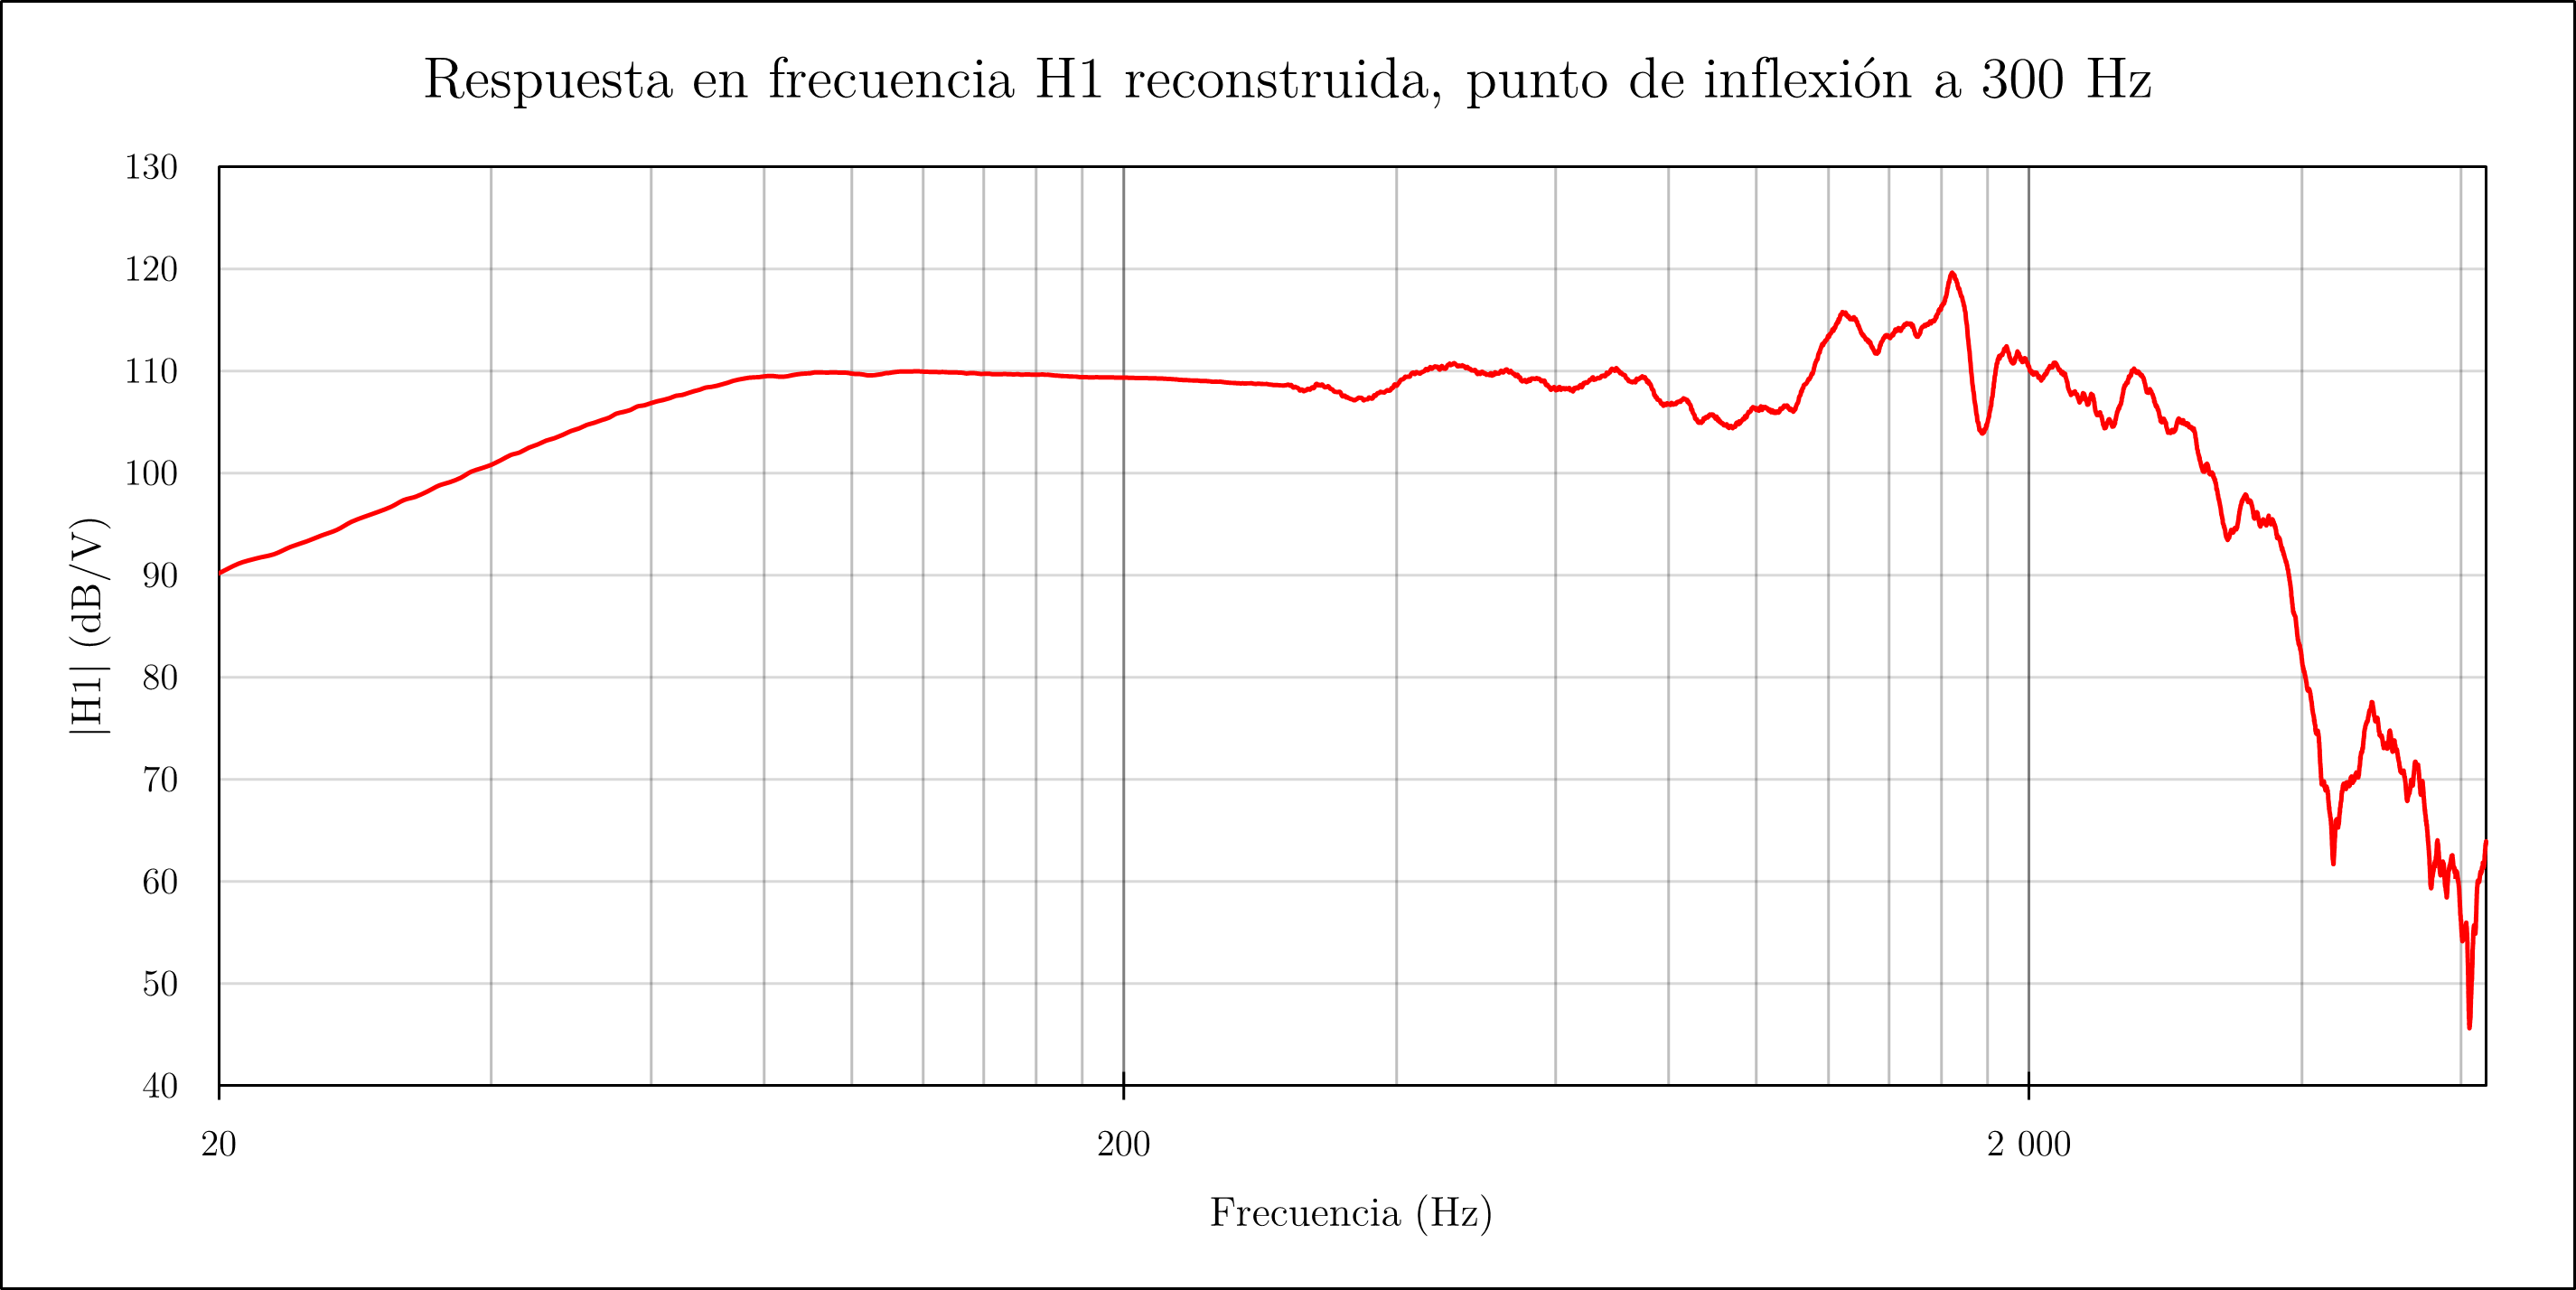
\includegraphics[width=0.8\linewidth]{h1_reconstruida.png}
  \caption{Respuesta anecoica del \textit{woofer} reconstruida a partir de las medidas de campo cercano y lejano.}
  \label{fig:h1_reconstruida}
\end{figure}

\subsubsection{Adjuntar las respuestas medidas del sistema de altavoces de tres vías con los filtros de cruce (polaridad correcta, inversión de polaridad del midrange, desplazamiento del tweeter...). Explicar el porqué de las diferencias entre curvas y por qué esas diferencias se producen sólo a determinadas frecuencias.}

Lo primero que se observa al analizar la \autoref{fig:tres_medidas} es que el sistema tiene una mala respuesta en general, en el sentido de que no es plana. Para ello se debe observar la medida roja, que corresponde con el sistema en condiciones normales.

Al comparar esta con la medida en la que se invirtió la polaridad del \textit{midrange} (azul) se comprueba que la respuesta sufre severas pérdidas en torno a ambas frecuencias de corte $f_{c1} = \qty{850}{\hertz }$ y $f_{c2} = \qty{4.7}{\kilo\hertz }$. Es importante recordar que las frecuencias de corte son zonas de inflexión determinadas por el filtro de cruce pasivo, donde existen dos altavoces trabajando y aportando un mismo nivel. Entonces, las pérdidas de nivel se deben a que la inversión de polaridad del altavoz fuerza a comenzar su oscilación en sentido opuesto, generando una presión acústica de signo contrario a la presión generada por los diafragmas de los otros dos altavoces, provocando una cancelación de presiones y, por tanto, una pérdida de nivel. Por último, cuando la frecuencia de excitación se aleja suficiente de las frecuencias de corte, el nivel medido se corresponde con el nivel que produce un solo altavoz, ya que los otros dos no están trabajando o bien trabajan produciendo un nivel mucho menor.

La tercera medida (verde) se corresponde con la respuesta en frecuencia con polaridad del \textit{midrange} normal pero con un desplazamiento de \qty{3.65}{\centi\metre} con respecto al eje que conformaban los tres altavoces en situación normal de funcionamiento. Esta distancia se escogió porque se corresponde con media longitud de onda para la frecuencia de corte superior $f_{c2}$.
\begin{equation} \label{eq:delta_x}
  \Delta x = \frac{\lambda }{2} = \frac{c}{2f_{c2}} = \frac{\qty{343}{\metre \per \second}}{2 \cdot \qty{4.
      7}{\kilo\hertz }} = \boxed{\qty{3.65}{\centi\meter}}
\end{equation}

En este caso también se puede observar que el nivel medido es menor que en el primer caso, aunque solamente en torno a $f_{c2}$. Las pérdidas de nivel suceden por el mismo problema que acabamos de comentar: la suma de presiones en oposición de fase procedentes de dos altavoces que trabajan simultáneamente. Sin embargo, en este caso la oposición de las fases no sucede por una inversión de la polaridad, sino por el propio camino acústico que recorre cada onda sonora. Como hemos medido en campo lejano y suponemos que el desplazamiento del \textit{tweeter} ha sucedido en el eje de vibración de los diafragmas, la presión que aporta el \textit{tweeter} llega al micrófono en oposición de fase con respecto al \textit{midrange}.

\begin{figure}[htp]
  \centering
  \includegraphics[width=\linewidth]{tres_medidas.png}
  \caption{Medidas de la caja en situación normal (rojo), con la polaridad del \textit{midrange} invertida (azul) y con el tweeter desplazado \qty{3.65}{\centi\metre} (verde).}
  \label{fig:tres_medidas}
\end{figure}

\subsubsection{Adjuntar las funciones de transferencia módulo/fase de los filtros de cruce (caso de carga \qty{8}{\ohm}). Adjuntar en forma de tabla las frecuencias de cruce $f_{c1}$ y $f_{c2}$, las ganancias en $f_{c1}$ y $f_{c2}$ de los filtros que se cruzan, la fase relativa (o diferencia de fase) de las vías implicadas en cada frecuencia de cruce y las pendientes de ganancia/atenuación de los filtros en dB/oct y dB/dec.}

\subsubsection{Usando las curvas de impedancia eléctrica de entrada para el caso ``\textit{woofer} en caja hermética'', calcular por el método de Small $f_c, Q_{ec}, Q_{mc}, Q_{tc}, \alpha$ (relación de compliancias del sistema de caja acústica cerrada) y $V_{ab}$ (volumen acústico equivalente). Usar los datos del fabricante (página 110 del libro). Obtener también $\gamma$, la constante termodinámica de la caja. Dato: $V_b = \qty{0.158}{\metre\cubed}$.}

\end{document}
